\documentclass{article}

\usepackage{phdstyle}
\usepackage[numbers]{natbib}

\begin{document}

\section{Perturbation of the spin motion}
The spin precession axis of a particle involved in betatron motion precesses about the invariant spin axis defined on the closed orbit.

This precession can be observed in polarization data as a rapid, small-amplitude oscillation on top of the \emph{major effect} oscillation, which is caused by the spin precession about the invariant spin axis defined for the closed orbit (see Figure~\ref{fig:Py_fit_residual}). 

\subsection{Simulation}
For simulation, we used an imperfect FS lattice, with E+B elements randomly tilted about the optical axis by angles picked from the normal distribution $N(8\cdot 10^{-2}~\text{[rad]}, 10^{-2}~\text{[rad]})$. The systematic $\Theta_{tilt} = 8\cdot 10^{-2}$ radians was selected to ensure a high radial precession rate and reduce tracking time requirements.

We tracked an ensemble of 4,000 rays through this system, 1,000 of which had initial offsets from the reference particle in the $x$ coordinate, 1,000 in $y$, and 1,000 in both $x$ and $y$ simultaneously; another 1,000 were offset in $d := \sfrac{\Delta K}{K}$.

\begin{figure}[!h]
  \centering
  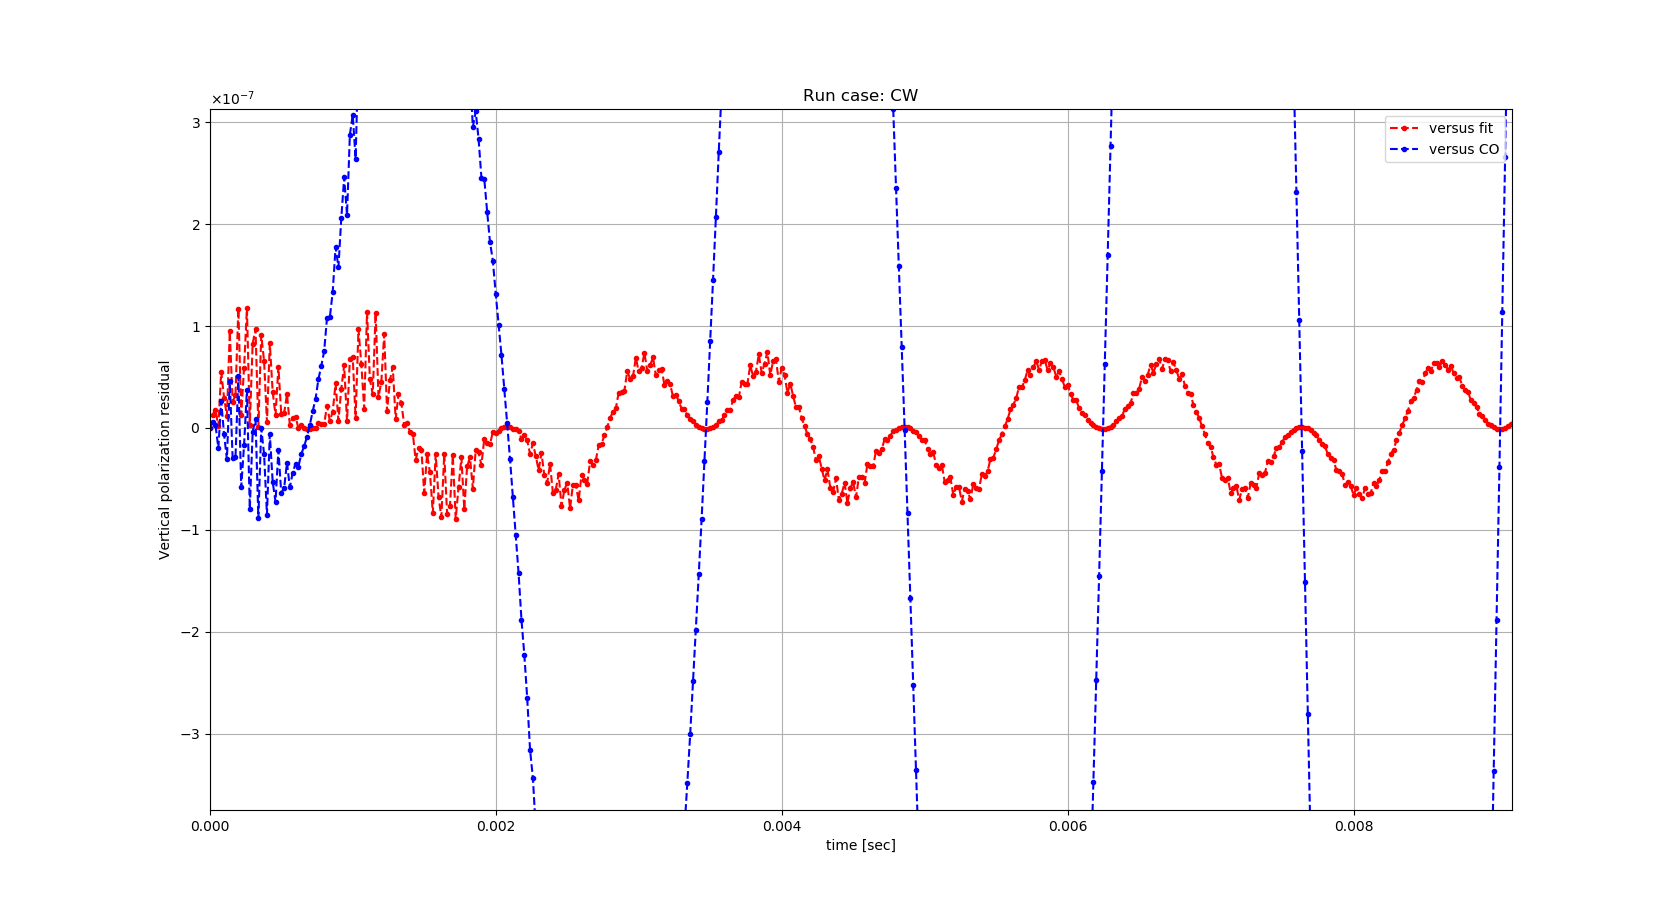
\includegraphics[width=\linewidth]{img/spin_axis_motion/Py_fit_residual}
  \caption{Vertical polarization residuals, computed as the difference between $P_y$ (data) and: (red) $\hat P_y$ (model prediction), (blue) $S_y^{co}$ (reference particle vertical spin component). The oscillations of the residuals are due to the rapid oscillations caused by the precession axis instability.\label{fig:Py_fit_residual}}
\end{figure}




\bibliography{PhDRefs}
\bibliographystyle{vancouver}


\end{document}

